\chapter{\label{ch4-software}Software} 

\minitoc

\section{Introduction}

Arguably, software is one of the most important aspects of modern-day astronomy. This is especially so for the Imaging Atmospheric Cherenkov Technique, due to its reliance on high-speed digitisers, the dependence of its sensitivity on how well one can reconstruct the shower, and the contrast between the rates of \gls{vhe} gamma-rays versus the hadron shower background.

In Chapter~\ref{ch3-architecture}, the data processing steps required to transition from the digitised waveform data obtain from the cameras to the science data release to the scientific community are described. In order transition through this chain, a number of software packages were developed, and are to be offered to \gls{cta} as in-kind contributions. This chapter provides an outline of the software packages involved in the processing pipeline for \gls{cta} and the camera commissioning for \gls{chec}. In cases where I have been involved in the development of the software, my contributions are also mentioned.

\section{TARGET Libraries}

A collection of libraries have been created to operate, read-out, and calibrate the cameras containing \gls{target} modules (i.e.\@ \gls{chec} and the \gls{sct} camera). Naturally, these are often referred to as the ``TARGET Libraries''. These low-level libraries were written in \cpp~as \final{check spaces afer cpp macro} they prioritise efficiency over flexibility. To enable the use of these libraries from the Python packages used in waveform reduction (described later in this chapter), a Python wrapper for these libraries is automatically generated during compilation through the utilisation of \pkg{\gls{swig}}\footnote{\url{http://www.swig.org/}}.

These libraries are presently stored on the \gls{cta}-SVN version control server, and installation instructions can be found at \url{https://forge.in2p3.fr/projects/gct/wiki/Installing_CHEC_Software}, provided you have permissions to the \gls{gct} Redmine.

\subsection{\pkg{TargetDriver}}
\vspace{-0.7em}
\noindent \hspace{\parindent} {\tiny URL: svn.in2p3.fr/cta/COM/CCC/TargetDriver/trunk \par}
\noindent \hspace{\parindent} {\tiny SVN revision: 32311 \par}

\noindent In order to operate the \gls{target} modules, the \pkg{TargetDriver} library is required. This \cpp~library configures the TARGET modules, and listens for the \gls{udp} packets containing the waveform data.

\subsection{\pkg{TargetIO}}
\vspace{-0.7em}
\noindent \hspace{\parindent} {\tiny URL: svn.in2p3.fr/cta/COM/CCC/TargetIO/trunk \par}
\noindent \hspace{\parindent} {\tiny SVN revision: 33028 \par}

\begin{figure}
  \centering
  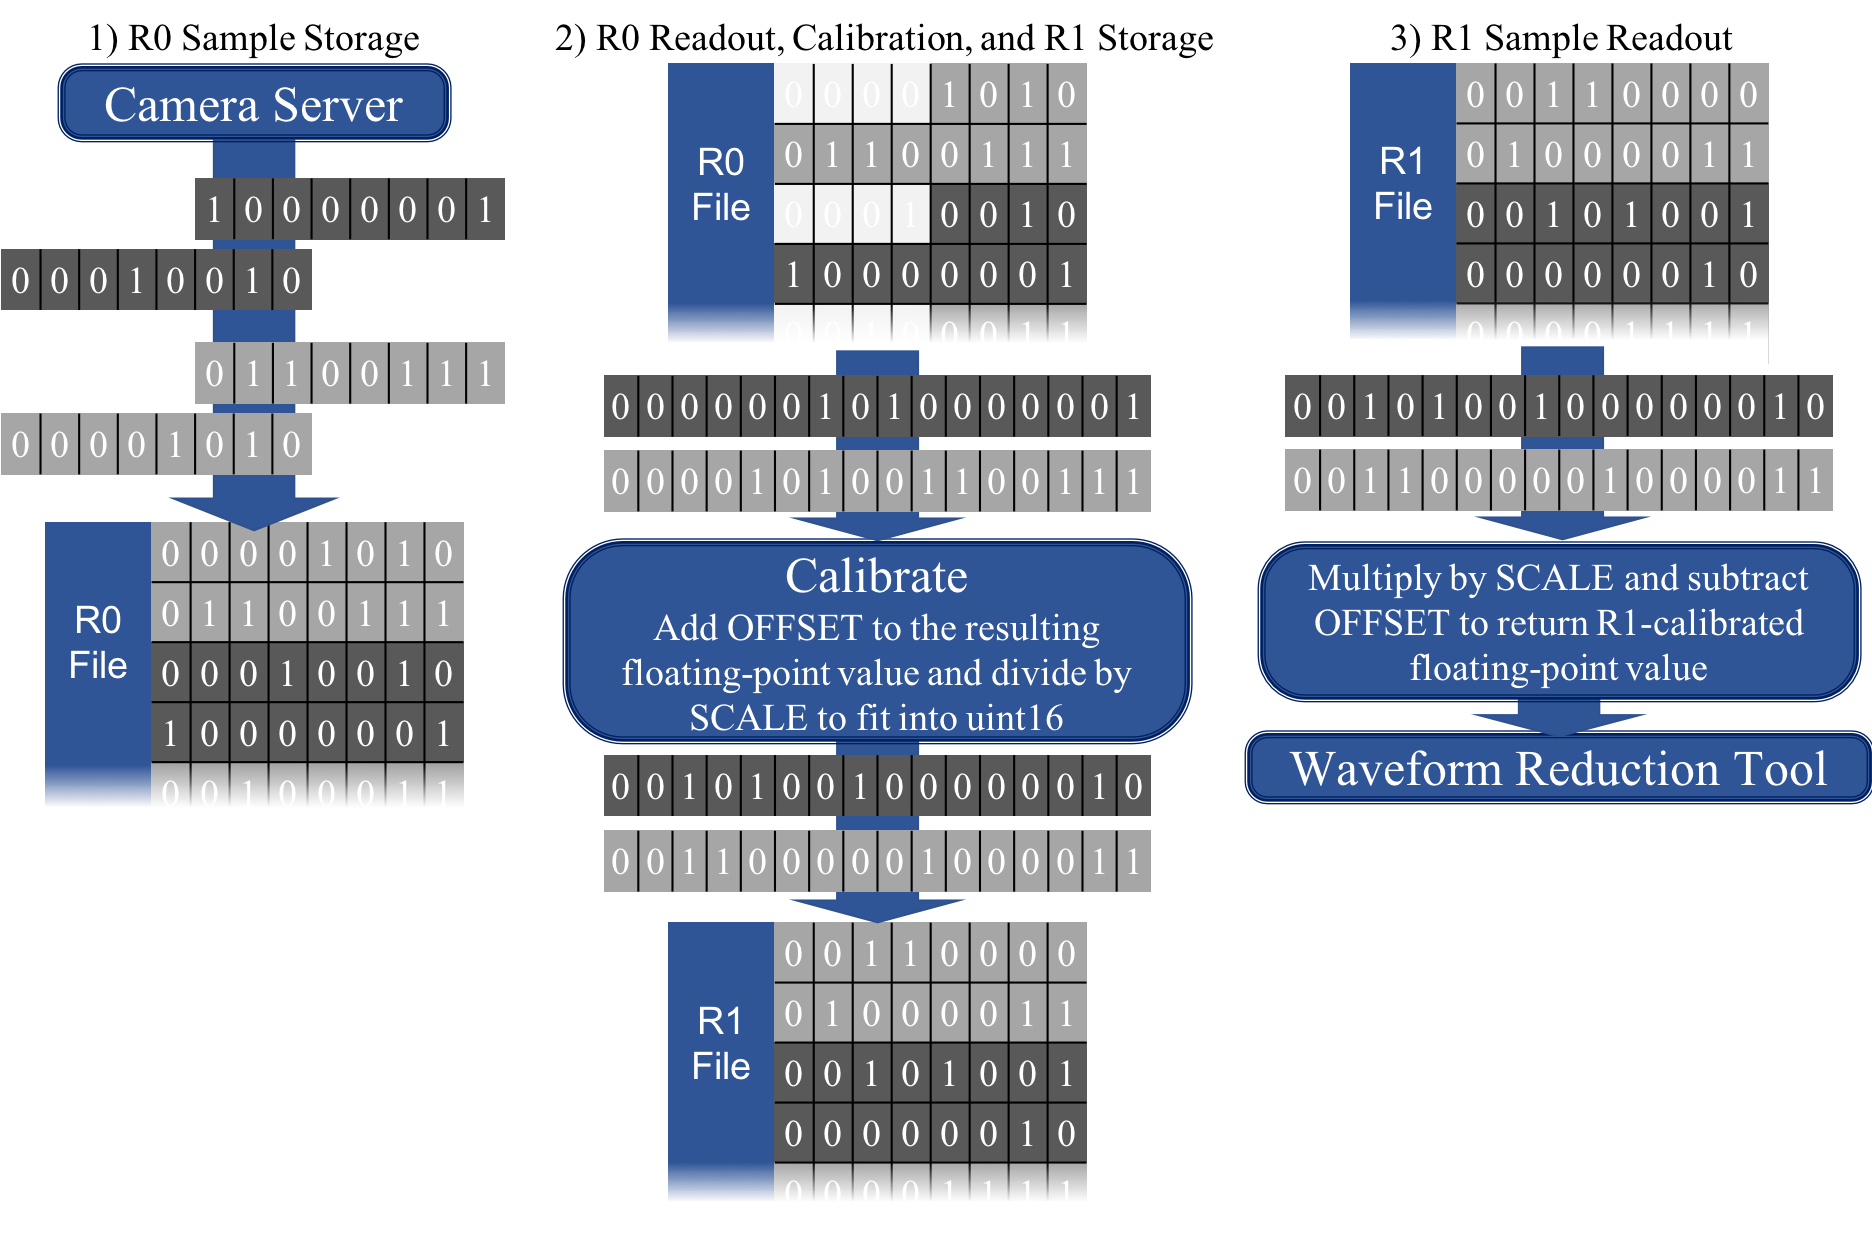
\includegraphics[width=\textwidth]{tio}
  \captionsetup{singlelinecheck=off}
  \caption[Simple overview of the data-flow for waveform samples within the TARGET libraries]{Simple overview of the data-flow for waveform samples within the TARGET libraries:
  \begin{enumerate}[label={\arabic*)}]
  \item 8-bit/char packets are sent from the TARGET FPGA and stored directly to file. A waveform sample is 12-bit, therefore the first four bits of the first 8-bit sample packet are used to indicate sample order.
  \item When reading a sample from the R0 TIO file, the first four bits are ignored, and the remaining twelve bits are combined into an unsigned 16-bit sample. The samples are passed to \pkg{TargetCalib} for calibration. The resulting calibrated floating-point sample is scaled and offset to fit into an unsigned 16-bit integer for storage.
  \item When reading a sample from a R1 TIO file, the entirety of the two 8-bit packets are kept and combined. The value is returned to floating-point format using the OFFSET and SCALE stored in the file header.
  \end{enumerate}
  
  Although only the samples are shown here, all other waveform data is also sent along this stream, including ASIC and Channel number, indicating the start of a new waveform. 
  }
  \label{fig:tio}
\end{figure}

\noindent The file format used to store waveforms from the \gls{target} modules is a custom \gls{fits} format defined by \pkg{TargetIO}, hereby referred to as the \gls{tio} format. This format was created as a temporary solution as the official \gls{cta} format is yet to be defined. \gls{fits} was chosen as it is well known and uses a convenient library with extensive compatibilities with other programming frameworks/languages. As we wished to store the \gls{udp} packets with minimal data arranging, they are stored in a customised binary table inside the \gls{fits}. This is a non-typical use of the \gls{fits} format, and therefore makes it complicated to read with typical \gls{fits} readers. The \pkg{TargetIO} library is therefore always used to read and write waveform and header (information such as observation time) data to and from the \gls{tio} file. \gls{tio} files can either contain \textit{R0} (uncalibrated)  or \textit{R1} (low-level calibrated) waveform data. Each sample in a waveform is stored to file as an unsigned 16-bit integer. The raw waveform digital counts measured by the camera are serialised in an unsigned 12-bit integer format, and the data packets received from the \gls{target} \gls{fpga} are 8-bit in size, therefore the first 4 bits of a waveform sample inside an \textit{R0} \gls{tio} file are not used. When storing calibrated waveforms, the post-calibration floating-point sample is scaled and offset to fit the full 16-bit unsigned integer. These scale and offset values are stored in the file header and automatically applied to convert the sample back into floating-point format when read. Figure~\ref{fig:tio} demonstrates the data-flow processes involving the \gls{tio} files.

To ensure the full efficiency of the \cpp~library is exploited via the Python wrapper, I contributed the |WaveformArrayReader| class, which, when passed a contiguous block of memory (such as a \lstset{language=Python}|numpy.array|), promptly fills the array with the entire camera's waveform data for that event. For example, to read an \textit{R1} \gls{tio} file from Python using \pkg{TargetIO} directly:

\begin{lstlisting}[language=Python]
import numpy as np
from target_io import WaveformArrayReader

# Create the reader and get the number of pixels and number of samples from the header
reader = WaveformArrayReader("/path/to/file/Run17473_r1.tio")
n_pixels = reader.fNPixels
n_samples = reader.fNSamples

# Generate the memory to be filled in-place
waveforms = np.zeros((n_pixels, n_samples), dtype=np.float32)
first_cell_ids = np.zeros(n_pixels, dtype=np.uint16)  # Storage cell id for the first sample of the event per pixel

# Fill the arrays
event_index = 20
reader.GetR1Event(event_index, waveforms, first_cell_ids)
# `waveforms' array is now filled with entire event's waveform data
\end{lstlisting}

\subsection{\pkg{TargetCalib}}
\vspace{-0.7em}
\noindent \hspace{\parindent} {\tiny URL: svn.in2p3.fr/cta/COM/CCC/TargetCalib/trunk \par}
\noindent \hspace{\parindent} {\tiny SVN revision: 33028 \par}

\noindent To correct for the effects of the \gls{target} electronics on the waveforms, \pkg{TargetCalib} was built. I have been responsible for the development of this package for the majority of its lifetime. The calibrations performed by this library are detailed in Chapter~\ref{ch5-calibration}. This package has also been adopted by \gls{sct} recently. The main classes in the library include:

\lstset{language=C++}
\begin{description}
\item [\textbf{PedestalMaker}] Generates the \textit{Pedestal} calibration file.
\item [\textbf{TfMaker}] Generates the \textit{Transfer Function} calibration file.
\item [\textbf{Calibrator}] Applies the aforementioned calibration files to the waveform samples.
\item [\textbf{Mapping}] Handles the files containing the camera's pixel mapping, and provides an interface to the information. This class is necessary due to the non-intuitive mapping between physics pixel position, and order of pixel readout (Figure~\change{figure showing the pixel positions, camera or module?}). Most commonly, this class is utilised for the plotting of camera images. The class is compatible with the mapping of any square-pixel telescope, and customisable to provide the mapping of the pixels in a single module, the mapping of the superpixels, the mapping of the modules, or the neighbours to a pixel/superpixel/module. This class will be deprecated once the central \gls{cta} database of telescope configurations exists.
\item [\textbf{CameraConfiguration}] Provides an interface to certain camera-version dependant variables. Currently the variables that might change with camera-version (stored in the \gls{tio} file header) include number of storage cells, pixel mapping, and reference pulse shape. The correct version of the parameter is returned according to the camera-version provided, allowing for the automated processing of the data of different camera versions. This class will also be replaced by the central \gls{cta} database.
\end{description}

Efforts are being made to improve the \pkg{TargetCalib}'s (more specifically the |Calibrator| class's) efficiency in terms of both memory and processing time, as it will need to meet the \gls{cta} Requirements for \textit{Online Analysis} (Chapter~\ref{ch3-architecture}). It is possible that in the future there will be two separate |Calibrator| classes for the \textit{Online} and \textit{Offline Analyses} respectively.

\section{Monte Carlo Software}

An important aspect in modern \gls{iact} analysis is the utilisation of Monte Carlo simulations. Within \gls{cta} they are paramount in both the design of the array, to find the most cost-effective solution that enables the attainment of its scientific goals, and as a complement to observational data in order to reconstruct Cherenkov showers from \gls{iact} images. Two packages are typically used for the generation of the files containing simulated Cherenkov shower images: \pkg{\gls{corsika}} and \pkg{sim\_telarray}.

\subsection{\pkg{CORSIKA}}
\vspace{-0.7em}
\noindent \hspace{\parindent} {\tiny URL: \url{https://www.ikp.kit.edu/corsika/} \par}
\noindent \hspace{\parindent} {\tiny Version: 6.99 \par}

\begin{figure}
  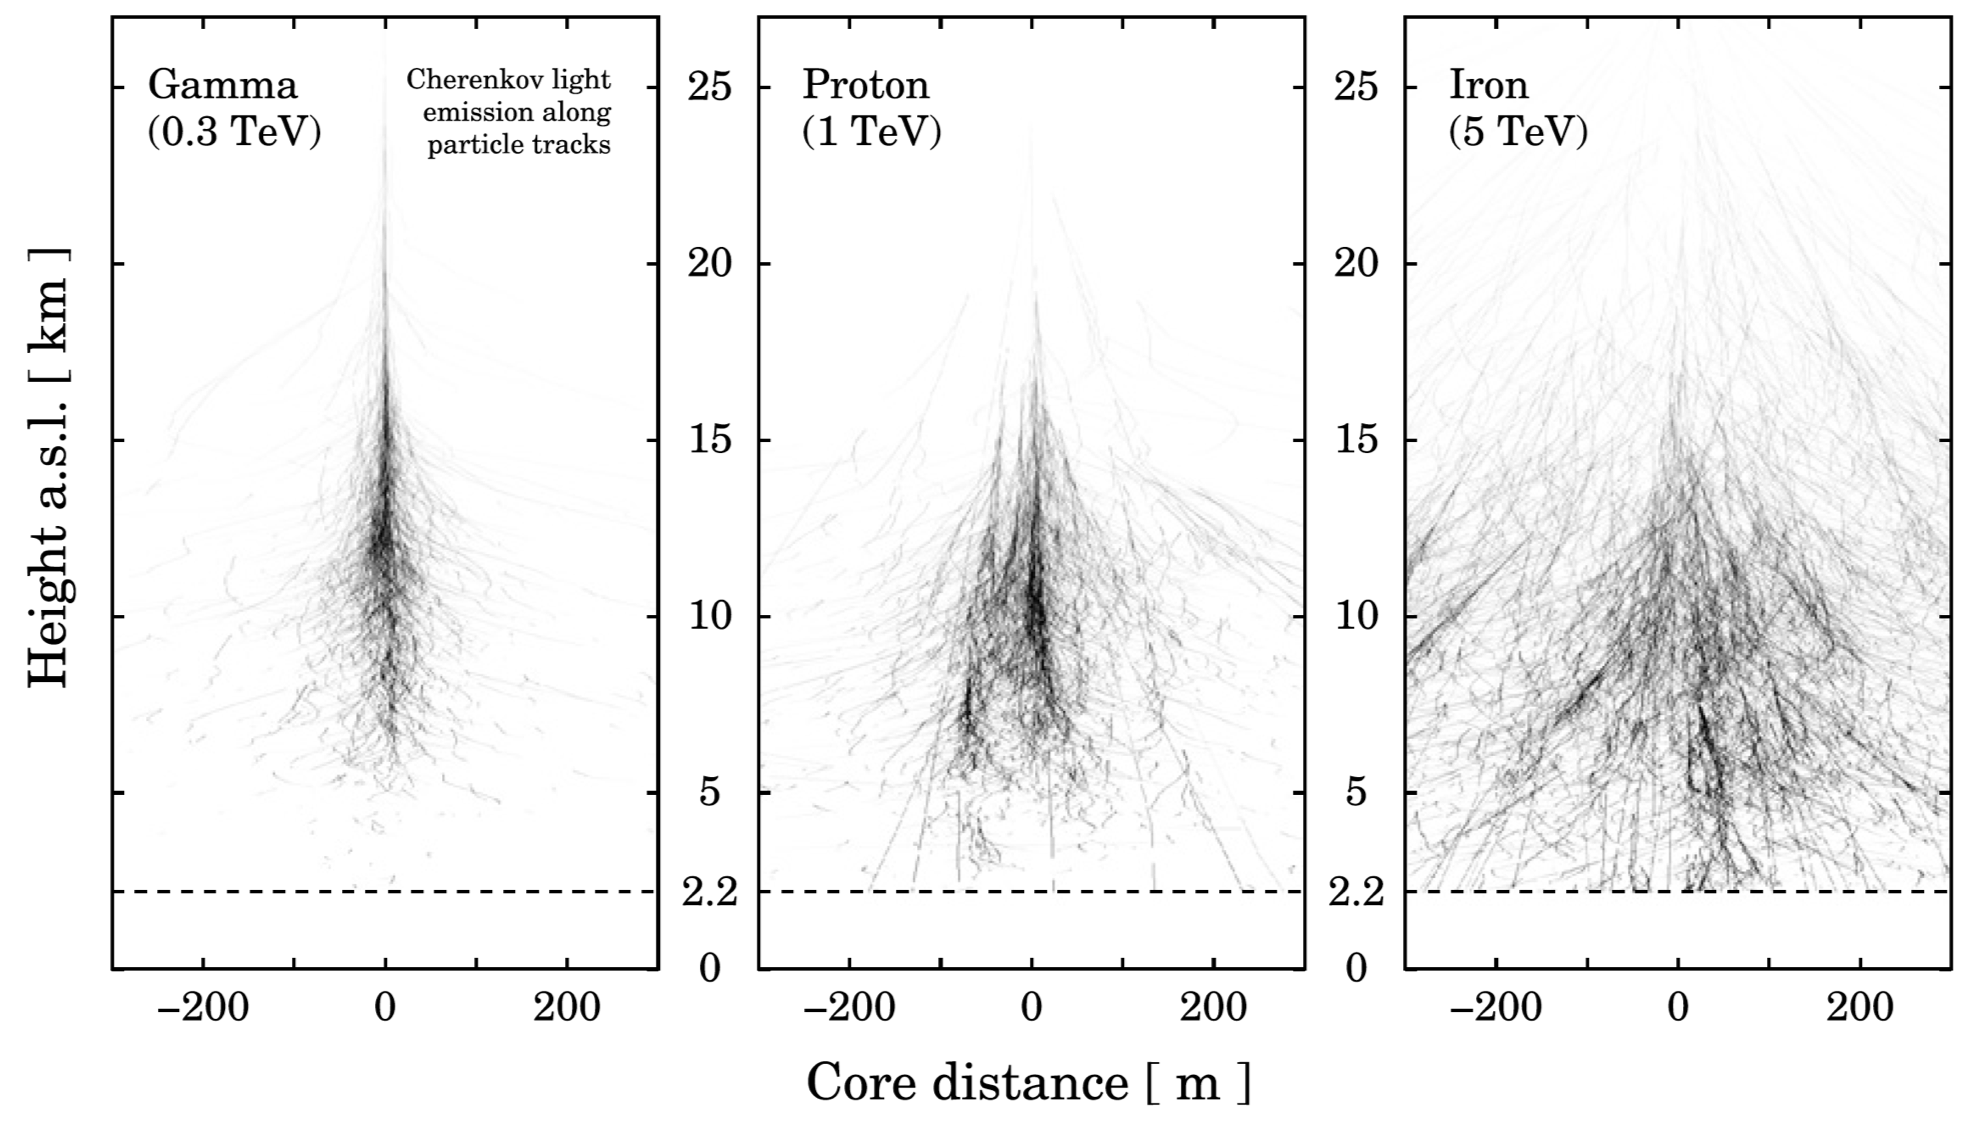
\includegraphics[width=\textwidth]{corsika}
  \caption[\pkg{CORSIKA} extensive air shower simulations.]{Cherenkov light production simulation from extensive air showers simulated by \pkg{CORSIKA}, for different primary particles for a site at \SI{2200}{m} altitude. Darkness of the particle tracks shown increases with increasing emission of Cherenkov light \cite{Bernlohr2008}.}
  \label{fig:corsika}
\end{figure}

\noindent Originally developed for the \gls{kascade} cosmic-ray experiment, the \pkg{CORSIKA} package is ``a program for detailed simulation of extensive air showers initiated by high energy cosmic ray particles'' \cite[][p. i]{heck1998corsika}. Given a specified astrophysical primary particle (protons, light nuclei, photons), the simulation tracks the particle, its interaction products, and its secondary decay products through the atmosphere, using the latest in hadronic and leptonic interaction models. It can also simulate the Cherenkov photon production produced by the superluminal products. In combination with the \gls{iact} extension package written by \textcite{Bernlohr2008}, these Cherenkov photons are tracked to a ``fiducial sphere'' surrounding the telescope, while including atmospheric refraction and absorption effects (Figure~\ref{fig:corsika}). Photons emitted at angles away from the telescope can be ignored to reduce the computational cost of this tracking. Photons are also simulated in bunches as opposed to individually to aid efficiency. The philosophy behind the development of \pkg{CORSIKA} is to provide an evolving package which accumulates the expertise from various experiments with connections to high energy and air shower physics. Due to the complexity involved in simulating extensive air showers, this is an attractive approach to minimise effort and errors, and ease the comparison of simulation results between experiments. As a result, \pkg{CORSIKA} is the most extensively used air shower simulation package in \gls{vhe} astrophysics. Experiments other than \gls{cta} that utilise \pkg{CORSIKA} include (but are not limited to) \gls{hess}, \gls{veritas}, \gls{magic}, and \gls{hawc}.

\subsection{\pkg{sim\_telarray}}
\vspace{-0.7em}
\noindent \hspace{\parindent} {\tiny URL: \url{https://www.mpi-hd.mpg.de/hfm/CTA/MC/Software/} \par}
\noindent \hspace{\parindent} {\tiny Version: 2018-06-12\_testing \par}

\noindent The second component in simulating the \gls{cta} observations of air showers is the simulation of the instrument's response to the Cherenkov photons resulting from the \pkg{CORSIKA} output. This includes the optical ray-tracing of the Cherenkov photons from where they impacted the ``fiducial sphere'' in \pkg{COSIKA} through the telescope's optics, the conversion of the photon into an electron by the sensors photocathode, the activation of the camera's trigger, and the digitisation of the resulting signal. The \pkg{sim\_telarray} package, developed by \textcite{Bernlohr2008} for \gls{hess}, has been adopted and developed to reproduce the \gls{cta} telescopes response to Cherenkov light in the Monte Carlo simulation chain.

Also included within the \pkg{sim\_telarray} package is the \pkg{light\_emission} package. This simple simulator produces \pkg{CORSIKA} output files for simple illumination cases. For example, one can simulate the uniform illumination of the camera focal plane. Therefore, using this \pkg{CORSIKA} output file as input to \pkg{sim\_telarray} will reproduce the illumination profiles often used in lab tests during the camera commissioning phase. This is especially useful in the Monte Carlo verification and validation process, discussed in Chapter~\ref{ch7-performance}.

\change[inline]{Talk about other simulation packages? GrOptics, KASKADE, SENECA, MOCCA}

\section{Reduction Tools}
\lstset{language=C++}

Tools used to process the waveforms in order to either characterise the camera or progress down the data-level chain (Figure~\ref{fig:dataflow}) are often referred to as ``reduction tools''. Within the \gls{chec} group we utilise Python for all of our waveform reduction. We made this choice due to its high popularity for data science and signal processing and its extensive library of statistical and numerical packages. The most important examples of these packages include:

\begin{description}
\item [\pkg{NumPy\footnotemark}] \footnotetext{\url{http://www.numpy.org/}} Enables the efficient processing of numerical data. This is accomplished using their powerful N-dimensional array object known as a |numpy.array| \cite{VanderWalt2011}. At the lowest level, a |numpy.array| is a contiguous block of memory much like an array in C. However, NumPy defines many statistical methods which utilise optimised low-level C and Fortran operations to process the contained data in the most efficient way possible, often performing better than handwritten C or Fortran.
\item [\pkg{SciPy\footnotemark}] \footnotetext{\url{https://www.scipy.org/}} Expands on the operations one can perform on the |numpy.array| object, providing an extensive amount of functionality useful for scientific computing, including statistical operations, interpolation, and signal processing.
\item [\pkg{Astropy\footnotemark}] \footnotetext{\url{http://www.astropy.org/}} Developed by the astronomy community to consolidate various common astronomy procedures into a single package. 
\item [\pkg{Pandas\footnotemark}] \footnotetext{\url{https://pandas.pydata.org/}} Provides high-performance, easy-to-use, table-like data structures known as a |pandas.DataFrame|. Each column in the table can be processed as a |numpy.array|.
\item [\pkg{Matplotlib\footnotemark}] \footnotetext{\url{https://matplotlib.org/}} Supplies extensive 2D plotting capabilities for Python, and is compatible with |numpy.array| objects.
\end{description}

Different reduction packages may be designed with different purposes, but each can potentially import methods from another, which is especially simple to do when developing in Python. Although many other \gls{cta} groups have also adopted Python for their waveform reduction software, it is not a standard across \gls{cta}.

\subsection{\pkg{ctapipe}}
\vspace{-0.7em}
\noindent \hspace{\parindent} {\tiny URL: \url{https://github.com/cta-observatory/ctapipe} \par}
\noindent \hspace{\parindent} {\tiny Version: 0.6.0 \par}

\noindent Waveform data from each \gls{cta} telescope must be processed and the results combined using standardised approaches, such that the data at each processing stage is compatible with the next, and the resulting reduced data and shower reconstruction is of optimum quality. This was the motivation behind the design of the \textit{Data Processing Level} architecture (Section~\ref{section:data_levels}). The most reliable way to ensure this architecture is adhered to was to create a single data processing pipeline with the capability to transform \textit{DL0} waveforms into \textit{DL2} reduced shower parameters. The prototype that has been developed among members of the \gls{cta} Consortium for this purpose is \pkg{ctapipe}.

The majority of pipeline frameworks in \gls{vhe} astronomy utilise what we refer to as a ``bottom-up'' approach, where the algorithms are written in low-level languages such as C or \cpp, and perhaps interfaced with a high-level language such as Python. Examples of this are the Data Acquisition system in \gls{hess} \cite{Balzer2014}, and the \gls{aerie} framework in \gls{hawc} \cite{Abeysekara2018}. Contrary to this, the \pkg{ctapipe} framework utilises a ``top-down'' approach, where algorithms are first written in Python. Through the utilisation of \pkg{NumPy}, the majority of these Python algorithms will process data at exceptional rates, removing the need to write complex low-level code. Additionally, as mentioned previously, there exists a wide scientific-computing community in the world of Python, contributing their collective knowledge into open-source packages. Within \pkg{ctapipe} we utilise this rich resource and benefit from the open-source model: reducing time wasted reproducing existing methods, and limiting the potential for bugs to go undiscovered. However, in some complicated applications which perform very specific tasks, \pkg{NumPy} is too generalised for the algorithm to perform adequately. In these cases the following options are available in Python:

\begin{description}
\item [\pkg{Numba}] A Python compiler, either prior to runtime, or ``just-in-time''. Allows for the optimisation of array-oriented and maths-heavy Python code without the need to switch to a different language.
\item [\pkg{Cython}] Converts Python code into C code, which can then be compiled for easy optimisation. Also enables the easy importing of external C or \cpp~code into Python.
\item [C/C++] The algorithm could instead be completely written in C or \cpp. The code can be included into Python in a variety of ways. One way is the use of \pkg{Cython}. A second possibility is the utilisation of \pkg{\gls{swig}}, as we have done for the \gls{target} libraries.
\end{description}

In the remainder of this subsection, I will describe the most important areas of \pkg{ctapipe} to which I have contributed.

\subsubsection{DataContainer}

\begin{figure}[t]
  \centering
  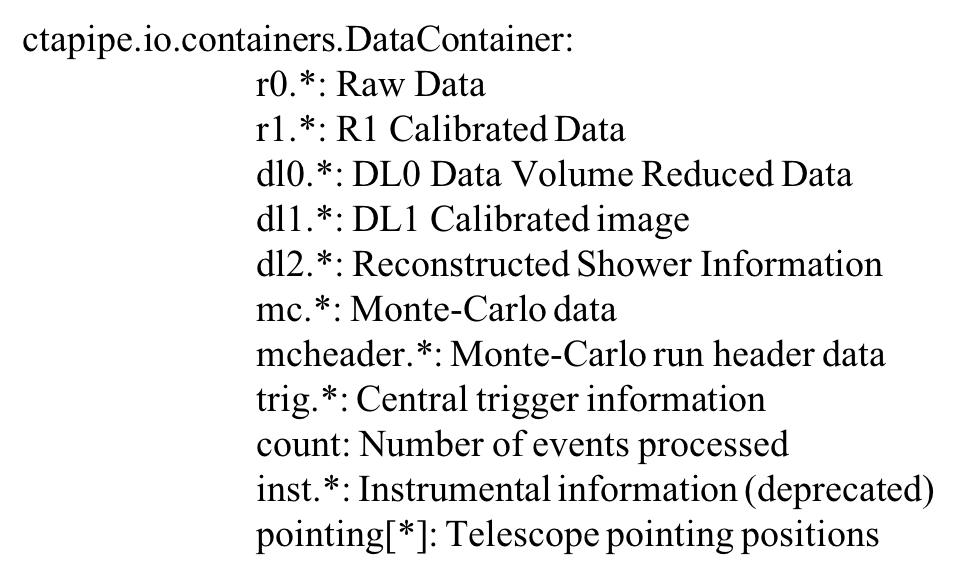
\includegraphics[width=0.9\textwidth]{datacontainer}
  \caption[Contents of the  {\protect \lstinline{ctapipe.io.containers.DataContainer}} object.]{Print result of a {\protect \lstinline{ctapipe.io.containers.DataContainer}} object, showing its contents.}
  \label{fig:datacontainer}
\end{figure}

As \pkg{ctapipe} must be capable of processing the data from any camera indiscriminately, one of the most important classes in \pkg{ctapipe} is the |ctapipe.io.containers.DataContainer|. This class can be filled from any data source, thereby allowing the same operations to be performed on the data irrespective of camera type. One of my contributions to \pkg{ctapipe} was to suggest that it would be logical for the contents of this class to closely follow the \gls{cta} data-level definitions (Section~\ref{section:data_levels}), as demonstrated in Figure~\ref{fig:datacontainer}. Therefore, in each stage of the data processing, the correct data level is read, and the following data level is filled. This also easily allows for different data levels to be saved to file, and to be read at a later time for further processing along the chain.

\subsubsection{EventSource}

\begin{figure}[t]
  \centering
  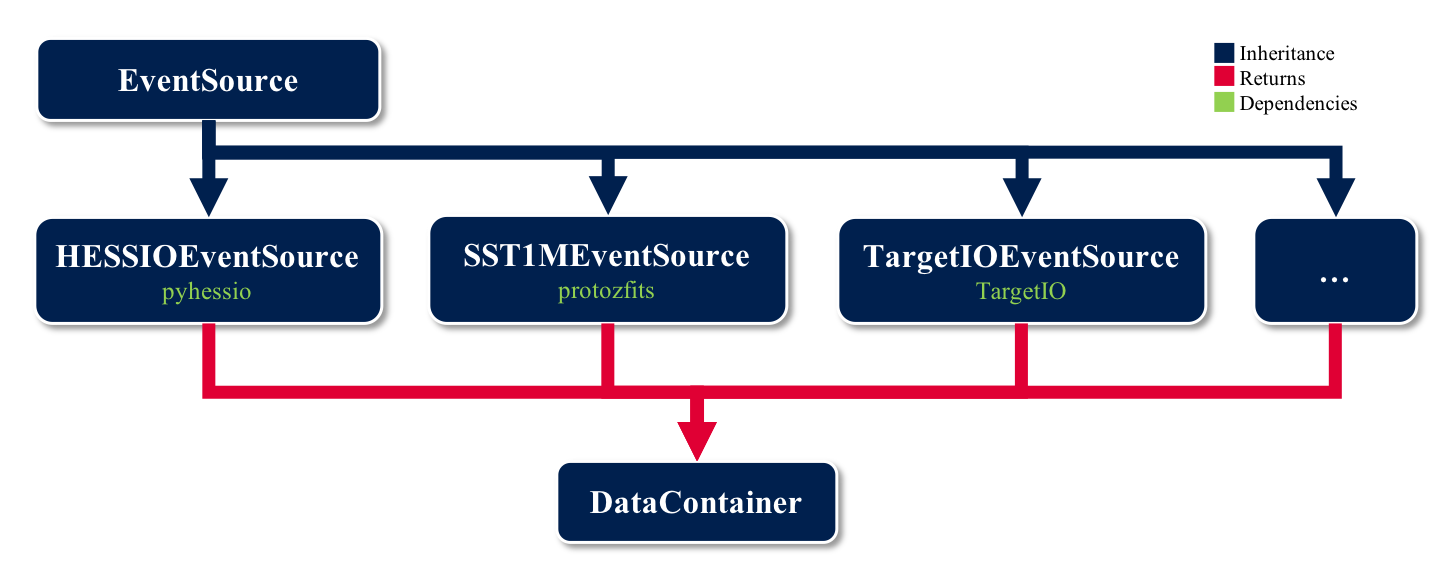
\includegraphics[width=\textwidth]{eventsource}
  \caption[Functional block diagram of the \lstinline{ctapipe.io.eventsource.EventSource} class.]{Functional block diagram of the \lstinline{ctapipe.io.eventsource.EventSource} class, showing the inheritance, dependencies, and object returned for a selection of the existing \lstinline{EventSource} classes.}
  \label{fig:eventsource}
\end{figure}

Presently in the development of \gls{cta}, a common file format has not yet been defined. Therefore, each camera currently uses their own data format for camera prototyping, such as the \gls{tio} format within \gls{chec}. Additionally, \pkg{sim\_telarray} stores the telescope simulation files in its own compressed data format, called HESSIO (for legacy reasons). In order for \pkg{ctapipe} to be fully prototyped, it must therefore be capable of reading in each of these file formats. One of my major contributions to \pkg{ctapipe} was the development of the |ctapipe.io.eventsource.EventSource| class. This class provides a base from which a new |EventSource| class can be created in order to add a file format to \pkg{ctapipe}'s compatibility list. For example, I also created the |ctapipe.io.hessioeventsource.HESSIOEventSource| and |ctapipe.io.targetioeventsource.TargetIOEventSource|. To create a new |EventSource| class, one simply has to define how the data is read from the file, into the |ctapipe.io.containers.DataContainer|. A dependency on the external custom camera software may exist for the reading of the file format. One must also create an |is_compatible| method for checking if the file supplied is compatible with the |EventSource|. The functional block diagram for the |EventSource| class is shown in Figure~\ref{fig:eventsource}.

\subsubsection{Factory}

\begin{figure}[t]
  \centering
  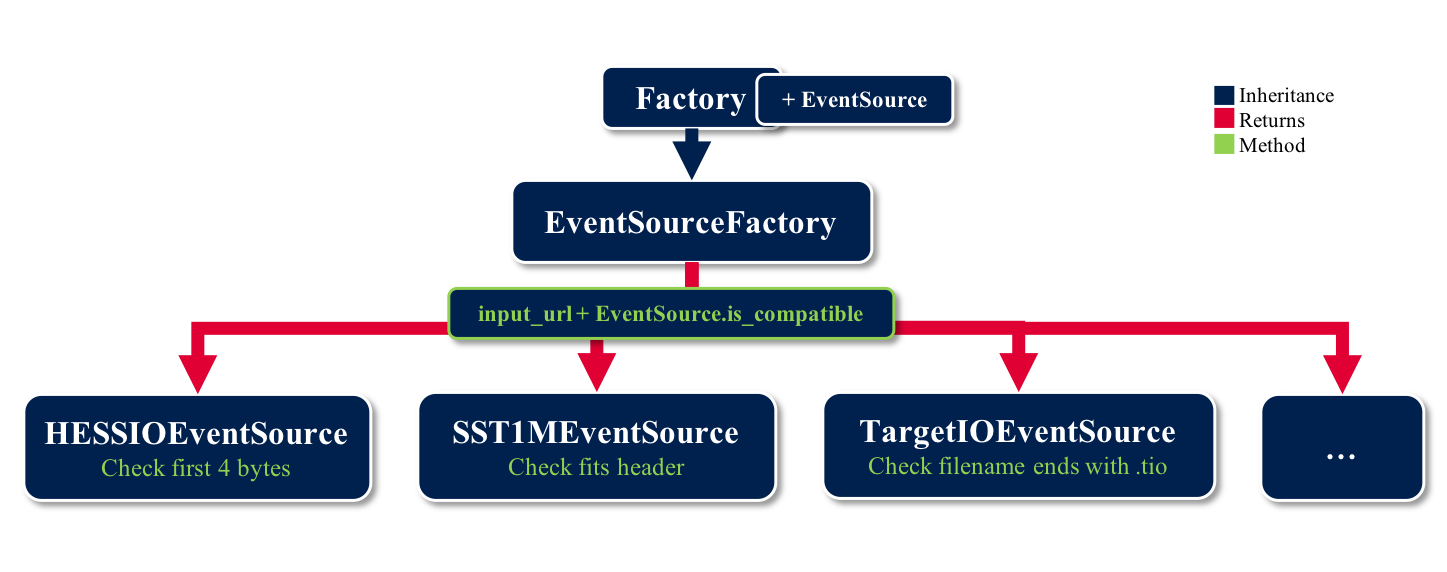
\includegraphics[width=\textwidth]{eventsourcefactory}
  \caption[Functional block diagram of the \lstinline{ctapipe.io.eventsourcefactory.EventSourceFactory} class.]{Functional block diagram of the \lstinline{ctapipe.io.eventsourcefactory.EventSourceFactory} class, showing the inheritance, the potential \lstinline{EventSource} classes that could be returned, and the methods used to assess the compatibility of the input URL with the \lstinline{EventSource}.}
  \label{fig:eventsourcefactory}
\end{figure}

Alongside the variety in file formats, their also exists a variety among \gls{iact} analysis techniques that are applicable to \gls{cta}, such as different charge extraction techniques or shower parametrisation approaches (Chapter~\ref{ch6-reduction}). Early in my involvement with \pkg{ctapipe} I identified the need for a design pattern that could enable the configuration of the processing chain at runtime, depending on user and file inputs. This approach needed to be clean and modular, otherwise such approaches can get very confusing and hard to maintain. As Python is a very flexible language, this problem was potentially easier to solve than if \pkg{ctapipe} was designed in a different languages. The accepted solution, of which I proposed and implemented, was to generate the |ctapipe.core.factory.Factory| class, which operates according to the ``factory method pattern'' \cite{johnson2005design}. By inheriting from the |Factory| class, one can design a factory that, when given a particular input, returns the corresponding class. The input can be designed to be anything, from a file path to a user's input on the command line. One example of a |Factory| is the |ctapipe.io.eventsourcefactory.EventSourceFactory| class (Figure~\ref{fig:eventsourcefactory}). Given an input URL, every |EventSource| is looped through, and the corresponding |is_compatible| static method is called. When |is_compatible| returns |True|, that |EventSource| is returned and used to read the file into the |DataContainer|. This functionality design makes reading any compatible file format into \pkg{ctapipe} extremely simple. The code snippet below demonstrates how to read a file and print the |event_id| for each event. It uses the helper function |ctapipe.io.eventsourcefactory.event_source| which internally handles the creation of an |EventSourceFactory| object. This snippet also demonstrates the simple functionality provided by the |EventSource| to easily loop through the events inside the file, irrespective of the file format.

\begin{lstlisting}[language=Python]
from ctapipe.io.eventsourcefactory import event_source
with event_source(url) as source:
   for event in source:
      print(event.r0.event_id)
\end{lstlisting}

\subsubsection{Calibration and Waveform Reduction in \pkg{ctapipe}}

\begin{figure}[t]
  \centering
  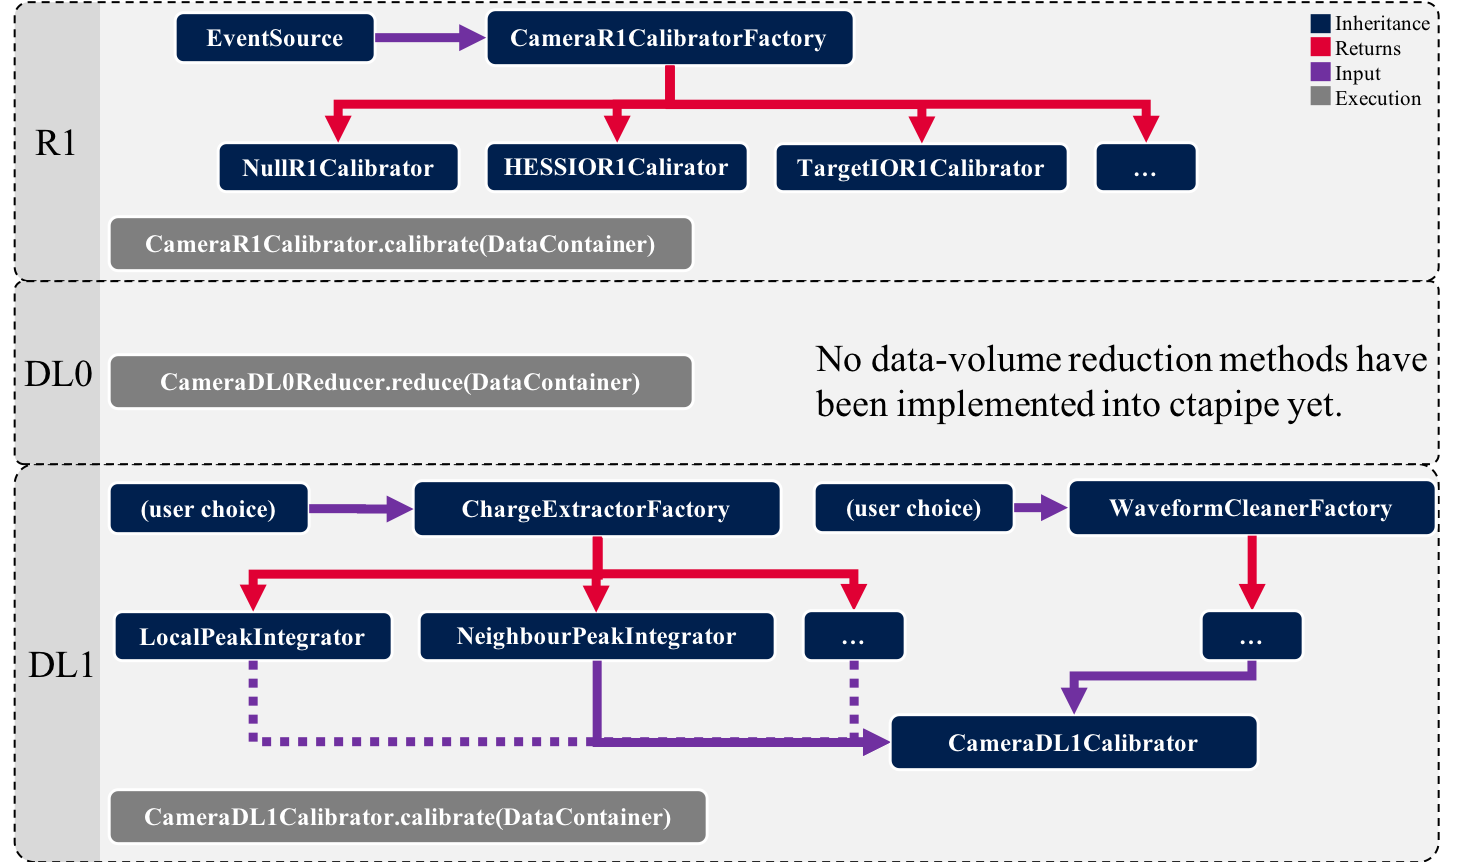
\includegraphics[width=\textwidth]{ctapipe_calib}
  \caption[Functional block diagram of the \pkg{ctapipe} low-level calibration classes.]{Functional block diagram of the \pkg{ctapipe} low-level calibration and waveform reduction classes (\textit{R1}, \textit{DL0}, and \textit{DL1}).}
  \label{fig:ctapipe_calib}
\end{figure}

Another major contribution of mine has been the development and maintenance of the calibration and waveform reduction pipeline within \pkg{ctapipe}. As with the |DataContainer|, each stage is split according to the data levels. Although the \textit{R1 Calibration} is a responsibility of the Camera Functional Unit (Section~\ref{section:data_levels}) and not the \gls{dpps}, it was concluded that it may be useful to be able to call \textit{R1 Calibration} methods from \pkg{ctapipe} during the prototyping phase. As shown in Figure~\ref{fig:ctapipe_calib}, the |ctapipe.image.charge_extractors.ChargeExtractor| classes are included within this scheme. The different charge extraction methods (Chapter~\ref{ch6-reduction}) are each selectable via the |ctapipe.image.charge_extractors.ChargeExtractorFactory|. An example of importing C code via \pkg{Cython} can be found for the |NeighbourPeakIntegrator|, as the loop over neighbouring pixels within a camera was too complex to optimally execute using \pkg{NumPy}.

\pkg{ctapipe} has reached a stage in its development at which full pipeline processing from waveform data into \glspl{irf} is possible, as it contains the common methods for \gls{iact} waveform reduction and shower reconstruction (see Chapter~\ref{ch6-reduction} for more details on these techniques). A first release of \pkg{ctapipe} is therefore intended later this year.

\subsection{\pkg{CHECLabPy}}
\vspace{-0.7em}
\noindent \hspace{\parindent} {\tiny URL: \url{https://github.com/cta-chec/CHECLabPy} \par}
\noindent \hspace{\parindent} {\tiny Version: ??\change{add version} \par}

\noindent It was decided within \gls{chec} that we need our own waveform reduction pipeline for camera commissioning and algorithm prototyping. The purpose of creating this package was to unify the analysis code in \gls{chec}, and supply a common method for file IO, thereby simplifying the reading of \gls{tio} files. A second primary motivation for this package was to provide an executable that would reduce the waveforms from \gls{tio} files into its signal, noise, and timing parameters, and store it into an accessible data format with no dependencies on the \gls{target} libraries or \pkg{ctapipe}. This therefore allows anyone within \gls{chec} to easily and immediately perform investigations on a dataset.

To meet these needs, I created the \pkg{CHECLabPy} Python package. This operates on the same principles as \pkg{ctapipe}, using a ``top-down'' approach, and utilising common scientific computing Python packages. By creating this package separately from \pkg{ctapipe}, we are able to freely develop algorithms that most likely will not be used in the final \gls{cta} array implementation, and therefore has no purpose within \pkg{ctapipe}.  However, the \pkg{CHECLabPy} has been designed with a similar coding style to \pkg{ctapipe}. Therefore, algorithms that are deemed useful to keep, such as the charge extraction approach we select to use for \gls{chec}, can easily be integrated into \pkg{ctapipe} in the future. The primary executable for reducing waveform data from \gls{tio} files is called |extract_dl1.py|, which allows a selection of |WaveformReducer| from the command-line using a similar factory method to the one I designed for \pkg{ctapipe}. The reduced parameters from the waveforms are then stored into a |pandas.DataFrame| object, which is then saved to disk in the HDF5\footnote{\url{https://support.hdfgroup.org/HDF5/}} file format.

\section{Science Tools}

Although not used in within this thesis, the science tools are important components to the \gls{cta} processing pipeline that are worthy of mention in this chapter. They will be provided to the scientific community, along with the \textit{DL3} data, by the \gls{suss} to support the science data analysis. This is an important aspect of the ``open-observatory'' operation of \gls{cta}.  As previous \gls{iact} experiments all built their own analysis tools, there exists no common tools within gamma-ray astronomy. Therefore, two independently-developed tools have been proposed for this purpose: \pkg{Gammapy} and \pkg{ctools}. Both packages intend to improve on the sharing-of-tools aspect of gamma-ray astronomy, through enabling the analysis of observational data from other experiments, and encouraging the standardisation of the data format used (\gls{fits}). Although the tools were developed to perform very similar operations, such as the construction of binned data products (including spectra, sky maps, and light curves) they have opposing design philosophies.

\change[inline]{any publications comparing the two yet?}

\subsection{\pkg{Gammapy}}
\vspace{-0.7em}
\noindent \hspace{\parindent} {\tiny URL: \url{https://github.com/gammapy/gammapy} \par}

\noindent Originally released under the name of \pkg{PyFACT} in 2011/2012, it explored the possibility of using the open-source Python model for \gls{vhe} data analysis, utilising the common scientific computing packages, \pkg{NumPy} and \pkg{SciPy} \cite{Deil2017}. Due to the amalgamation of the Python astronomy community to create \pkg{Astropy}, it was decided to create \pkg{Gammapy} as an \pkg{Astropy} affiliated package. This means that wherever possible, it uses functionality from \pkg{Astropy}, thereby benefiting from the entire Python astronomy community. This design philosophy is the same approach adopted by \pkg{ctapipe}. 

A Gammapy high-level analysis typically consists of \cite[][p. 4]{Deil2017}:
\begin{itemize}
\item selection of a data cube (energy and positions) around a sky position from all event lists,
\item computation of the corresponding exposure,
\item estimation the background directly from the data (e.g.\@ with a ring background model \cite{Berge2007}) or from a model (e.g.\@ templates built from real data beforehand),
\item creation of sky images (signal, background, significance, etc) and morphology fitting,
\item spectrum measurement with a 1D analysis or with a 3D analysis by adjusting both spectral and spatial shape of gamma-ray sources,
\item computation of light-curves and phasograms, search for transient signals,
\item derivation of a catalog of excess peaks (or a source catalog).
\end{itemize}

\subsection{\pkg{ctools}}
\vspace{-0.7em}
\noindent \hspace{\parindent} {\tiny URL: \url{http://cta.irap.omp.eu/ctools/index.html} \par}

\begin{figure}[t]
  \centering
  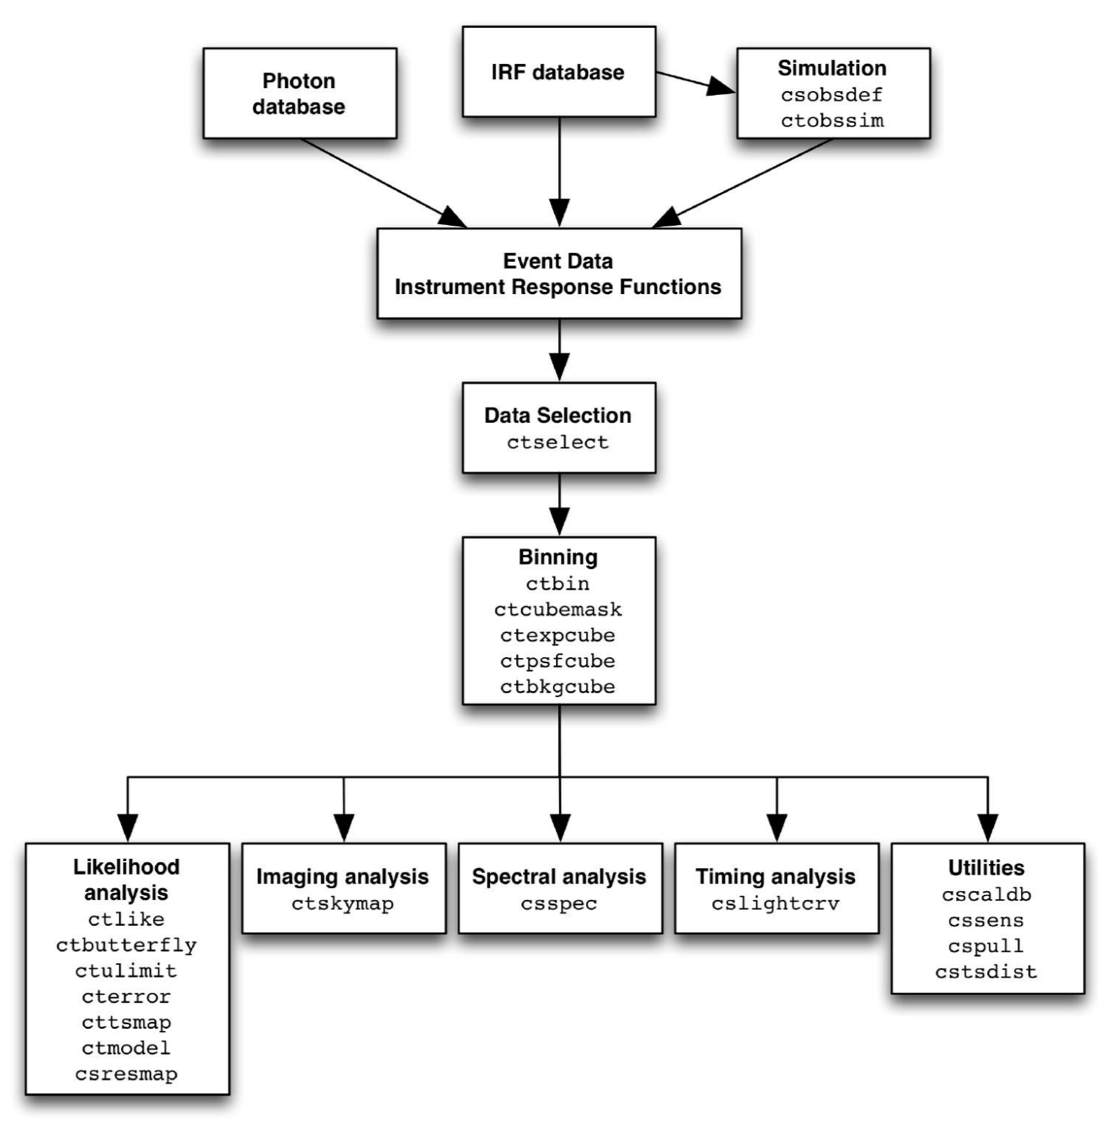
\includegraphics[width=\textwidth]{ctools}
  \caption[Overview of \pkg{ctools}.]{Overview of the contents of the \pkg{ctools} package \cite{Knodlseder2016}.}
  \label{fig:ctools}
\end{figure}

\noindent Conversely, the design philosophy of \pkg{ctools} is to strictly minimise dependencies as much as possible. The only dependency of \pkg{ctools} is the adjacently developed \pkg{GammaLib} \cpp~shared library, which contains ``all the classes, support functions, and some global variables that are needed to analyse gamma-ray event data'' \cite[][p. 2]{Knodlseder2016}. The advantage of this design lies in the complete independence from the maintenance of other libraries. If a dependency is no longer maintained in the future, many problems can arise in the form of incompatibilities, such those regarding operating systems or the updates inside the software package itself. However, the disadvantage of this design is the larger initial development effort required, and necessity to reimplement common methods from scratch.

Much like other science analysis frameworks in high-energy astronomy (e.g. Fermi Science Tools), \pkg{ctools} is a collection of tools that each perform a single, well-defined analysis step. These tools are written in \cpp, but can also be called directly from Python via the \pkg{SWIG}-generated interface. An overview of the \pkg{ctools} package is shown in Figure~\ref{fig:ctools}.

